\documentclass[../thesis.tex]{subfiles}
\graphicspath{{\subfix{figs/}}}
\begin{document}

\chapter{Methodology}
\label{ch:methods}

start with recap of previous chapters, into: ok so now what tools can we use. start with "old" way: classic linguistics, transition in ot computational and finish with complex systems stuff.
\cite{NguyenComputationalSociolinguistics2016}

different media to convey language
HERE written language exclusively, WHY: our methods, because that's what computers process better
SO we lose a lot of things that cannot be transcribed, or that are simply not because it would require considerable effort to do so  (accent, intonation), and access to spoken language is much more limited. also lose all non-verbal communication between human


Enormous amount of information exchanged through language. Data and metadata: . Someone's language tells a lot about them

methods with books "older data"

% data can say if model is wrong, but not if it's a good one: machine scientist stuff

\section{Data}

\subsection{What for}

\subsection{Traditional sources in linguistics}

\subsection{New sources from online media}

\subsection{The case of Twitter}

The biggest source of data we have used throughout this thesis is Twitter. Twitter is a micro-blogging website where people can register to share and view short posts called Tweets. These can be of three kinds:
\begin{itemize}
  \item a simple post that appears on the user profile and is shown on the homepage of
  all the users following this user, which is what people generally refer to with the
  term \emph{Tweet};
  \item a reply to another post, which is shown publically but only shown on the
  homepage of the users involved in the conversation;
  \item a repost to one's profile, to share a Tweet that is already posted (which can be
  one's own)called \emph{Retweets} (RT);
  \item a retweet but with some added text content commenting on the quoted post, called
  \emph{quote Tweets} (QRT);
\end{itemize}
The platform is called a micro-blogging website because those posts are limited to 280 characters (140 before 2017). % TODO more


\subsubsection{Accessing}
A major advantage of Twitter for academic research is how open the platform is to give access to its data to researchers. One can send automatic queries to Twitter for data through their public Application Programming Interface (API) \cite{TwitterAPI}. In these queries one can specify rules to for instance retrieve all the Tweets posted in a given country, in a given time period, or which contain some given text. All the Twitter data we have used throughout this thesis was  retrieved from the filtered stream endpoint of the Twitter API \cite{TwitterAPIa}. We show in \cref{fig:tweet_data} an example of the data we can have for each Tweet. 

\begin{figure}
  \centering
  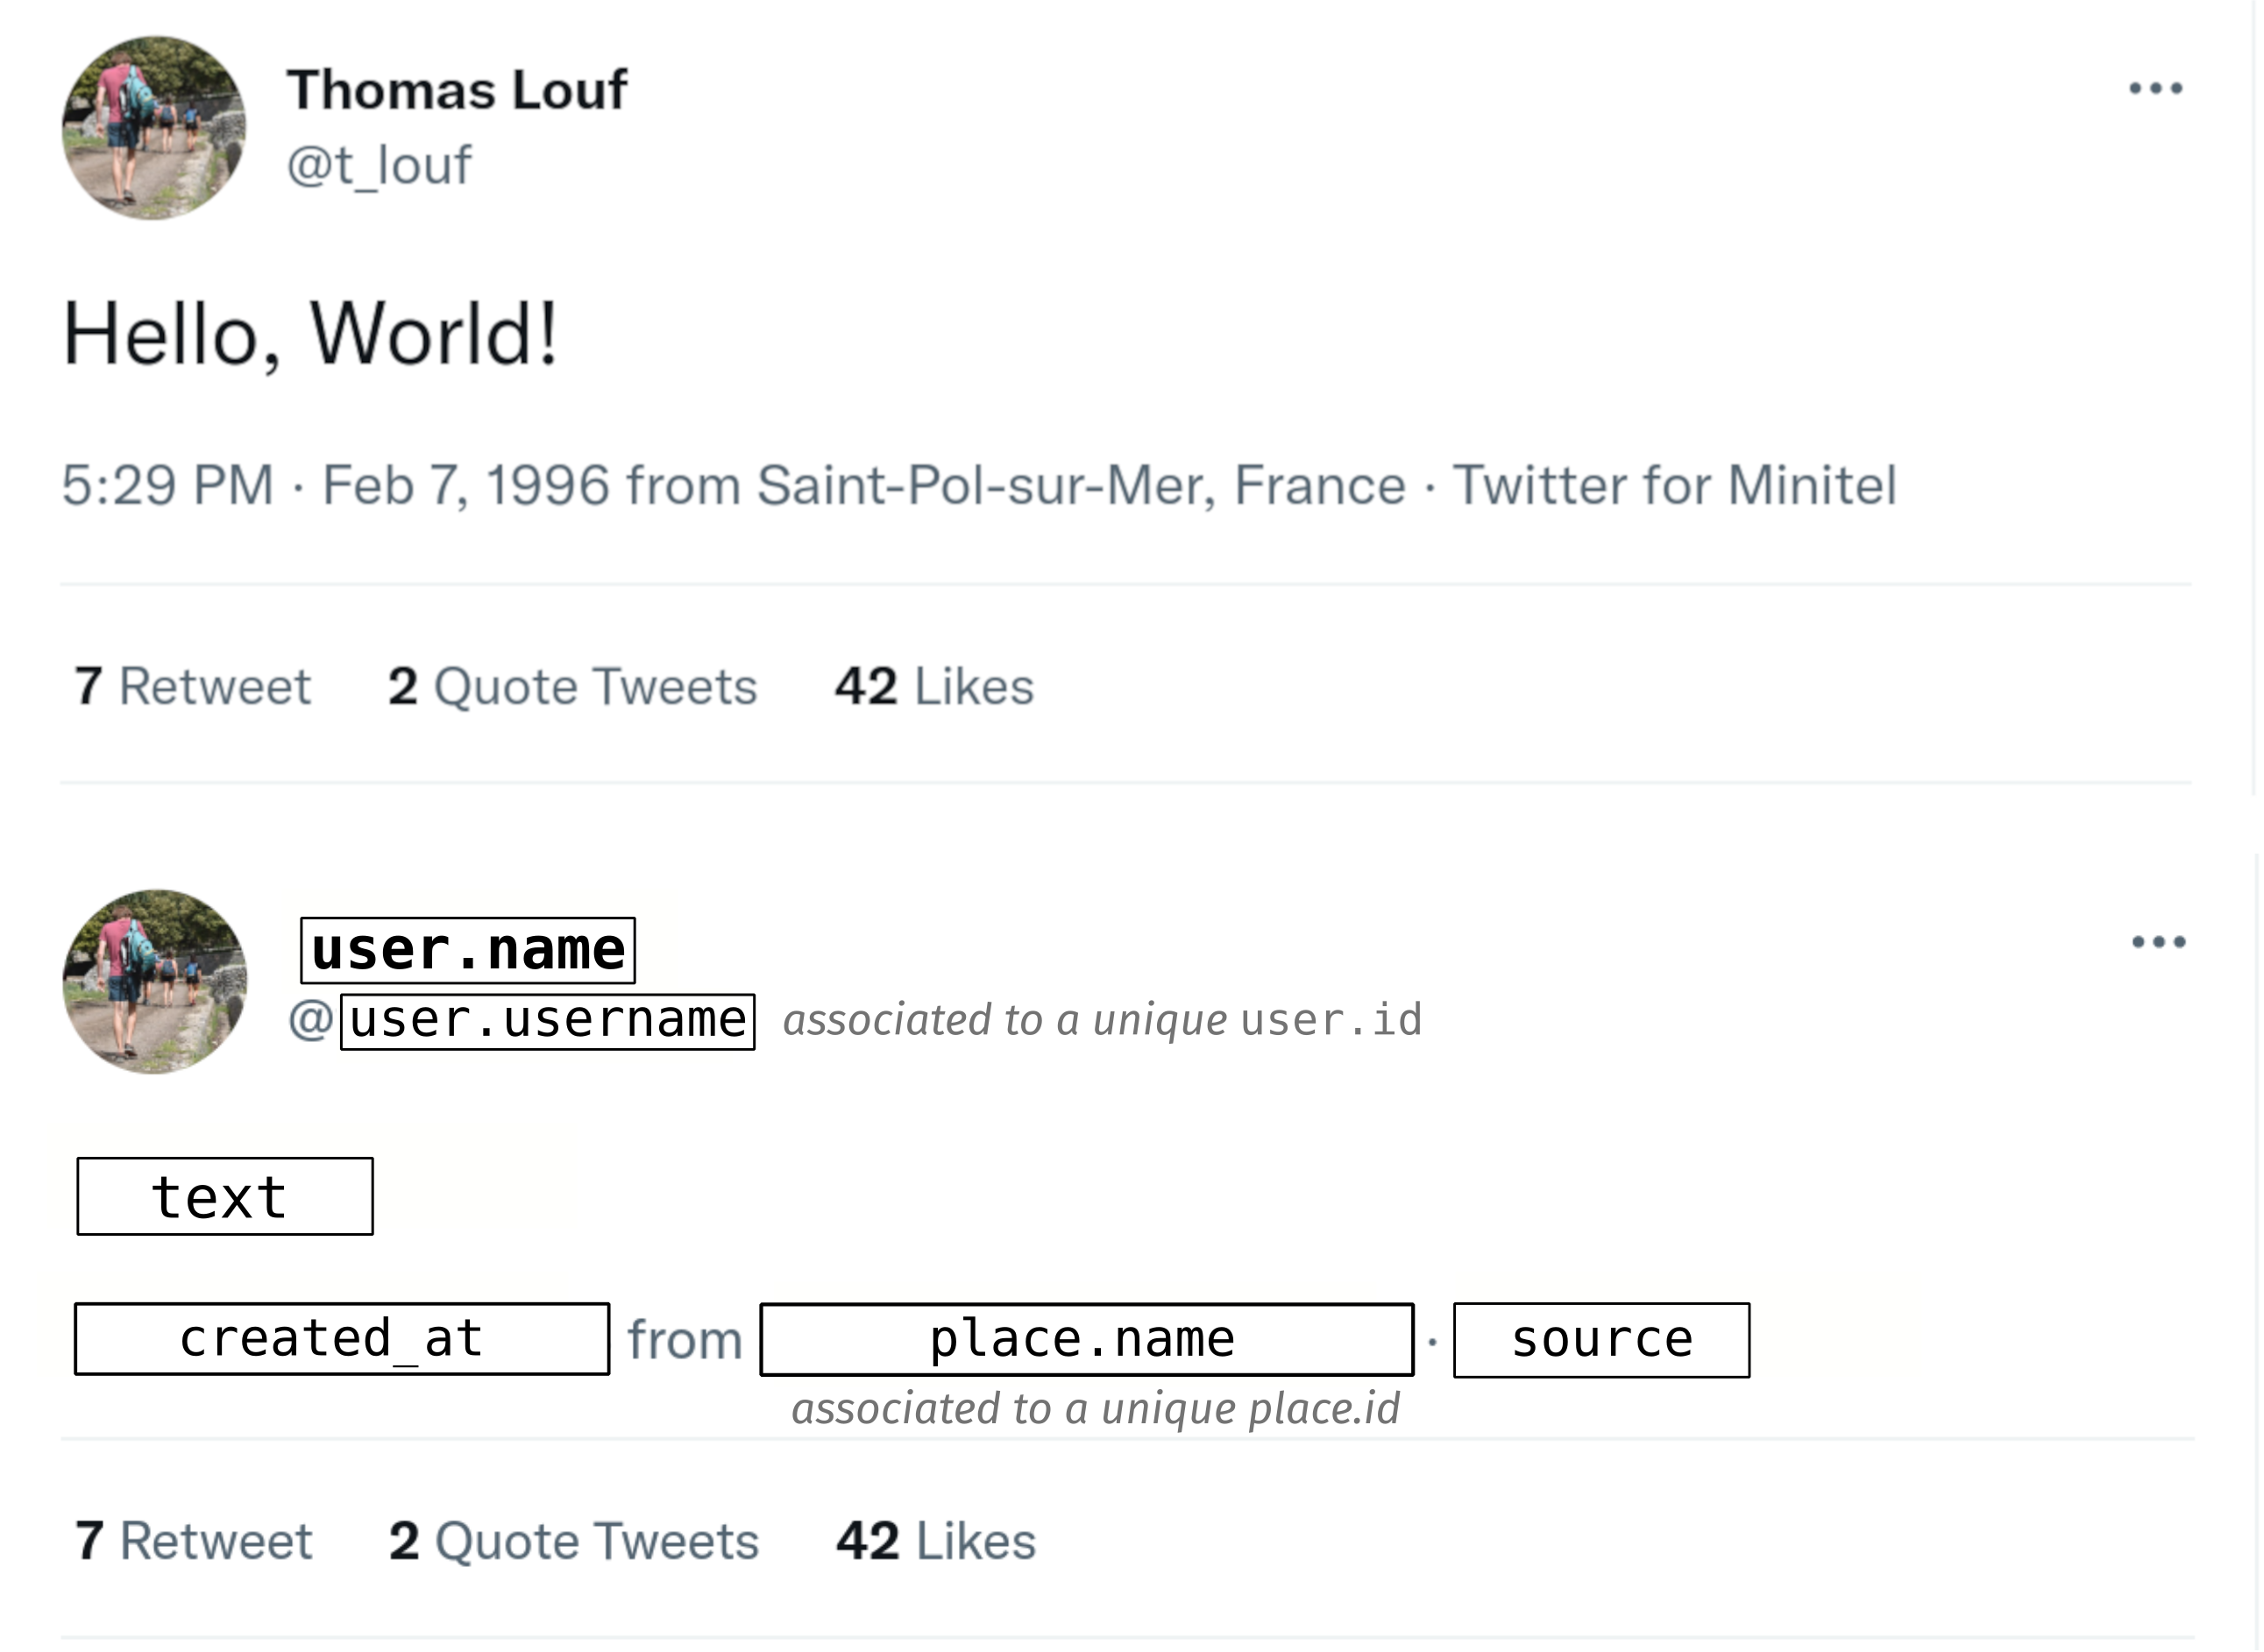
\includegraphics[width=0.8\textwidth]{tweet_fields.png}
    \begin{verbatim}
      {
        "id": "1234567890",
        "text": "Hello, World!",
        "created_at": "1996-02-07T04:29:05.000Z",
        "geo": {
          "place_id": "f68f3d5396bd681c",
          "coordinates": {
            "type": "Point",
            "coordinates": "[2.3295, 51.0249]"
          }
        },
        "source": "Twitter for Minitel",
        "user": {
          "id": "123",
          "username": "t_louf",
          "name": "Thomas Louf"
        }
      }
    \end{verbatim}
       \caption{An example Tweet as seen on Twitter, an annotated version with the name
        of the fields shown in boxes for the text of the Tweet and the visible metadata
        surrounding it. We also show how this Tweet data would be sent by the API, which
        is simply text formatted in a dictionary-like structure (JSON), with some of its
        keys corresponding to the annotated Tweet shown above.}
       \label{fig:tweet_data}
\end{figure}

There are two fields in these data that particularly interest us for the works we will
present in the next part and that need careful processing: the textual content of the
Tweet and its geotag.

\subsubsection{Text processing}
\label{sec:method_text_process}
Since we are interested in the speech produced by the user, we need to clean parts of
the text which cannot be considered as natural language production. Those are the URLs,
mentions of other users (in the form \texttt{@username}) and hashtags (in the form
\texttt{\#topic}). The latter is the least obvious. Hashtags are used on Twitter to
aggregate Tweets by topics. It is an important feature of Twitter, whose aim is to
enable users to easily find the Tweets of other users discussing similar topics,
inversely to make one's Tweets more discoverable by others, and to see real time trends
on the platform. Hence, there can be completely different motivations behind writing a
hashtag: to actually tag a Tweet with one or more topic, to promote the Tweet or simply
follow a trend. Thus, the content of hahstag can deviate significantly from normal
speech \cite{PageLinguisticsSelfbranding2012}. It is therefore safer to discard hashtags
entirely, which is no issue as long as it we can collect enough textual content without
them anyway. We actually made some measurements in our Tweets database. We took several
random samples of a million Tweets each, stripped them of URLs and mentions, and them
computed the ratio of characters within a hashtag compared to the total number of
characters left in those Tweets. We found that this proportion is consistently below
\SI{5}{\percent}. We thus consider the precaution of stripping hashtags off of Tweets
worth taking. In practice, all those elements are stripped off of Tweets using regular
expressions.

After cleaning the text, for what follows we then keep only the Tweets still containing
at least four words. The next important step that was crucial to all our works was to
infer the language the Tweets are written in. To do so, we leverage a trained neural
network model for language identification: the Compact Language Detector
\cite{SalcianuCompactLanguage2023}. It was designed as part of Chromium-based web
browsers to detect the language web pages are written in in order to make translation
suggestions to users, and it is now openly accessible. Its output is a language
prediction and the confidence of the model. Whenever we focus on a language, we thus
keep Tweets whichc are tagged in that language with a confidence above
\SI{90}{\percent}.

We have thus described the basic steps of text pre-processing that are recurrent in our
works. Out of it we get the Tweets for which we could reliably assign a language, and
the parts that are relevant to us.



\subsubsection{Infering geolocation}

\subsubsection{Caveats}
cover Twitter (biases but also basic technical details, API, what Tweet looks like), why remove HTs, blabla, language IDtion data driven analysis, cite Bruno papers eg

theoretical models: AS, MW 

finally computational methods, very general (data, PCA...)


\section{Models}

\subsection{What for}

\subsection{What kind}



\section{Source materials and tools}
Following the principles of open science, throughout my thesis, I have made all source
materials for my results openly accessible, whether they are codes\footnote{Hosted on
GitHub at \url{https://github.com/TLouf}} or datasets\footnote{Hosted on figshare at
\url{https://figshare.com/authors/Thomas_Louf/9441395}}, including this very
manuscript's\footnote{Hosted at \url{https://github.com/TLouf/phd-thesis}}. Equally importantly, I believe, I have strived to use almost exclusively free
and open source software in my work. I cannot realistically cite here all projects I
have relied on to carry out my work, but I can cite a few central ones. I wrote all my
code in the Python 3 programming language, using libraries such as
NumPy~\cite{HarrisArrayProgramming2020},
pandas~\cite{teamPandasdevPandas2020} or
GeoPandas~\cite{JordahlGeopandasGeopandas2020}. In their vast majority, figures
presented here were prepared with Matplotlib~\cite{HunterMatplotlib2D2007}, and
sometimes edited, or entirely drawn, with Inkscape\footnote{Available at
\url{https://inkscape.org}}.

This document was prepared using \LaTeX\ with the \texttt{classicthesis}
style\footnote{Hosted at \url{https://www.ctan.org/pkg/classicthesis}} developed by
Andr\'e Miede and Ivo Pletikosić, and the LaTeX Workshop extension\footnote{Hosted at
\url{https://github.com/James-Yu/LaTeX-Workshop}} of Visual Studio Code.
% managed the references cited in this work with Zotero https://www.zotero.org/


\section{Outline}



\end{document}
